\section{Data Analysis with De-Noising}

\subsection{Luminosity dependence}

Track reconstruction efficiency degrades with increased luminosity (incident beam current on the target) due to background
noise. The increased noise in the drift chambers results in failure of clustering algorithm to identify clusters from raw hits. 


\begin{figure}[!ht]
\begin{center}
 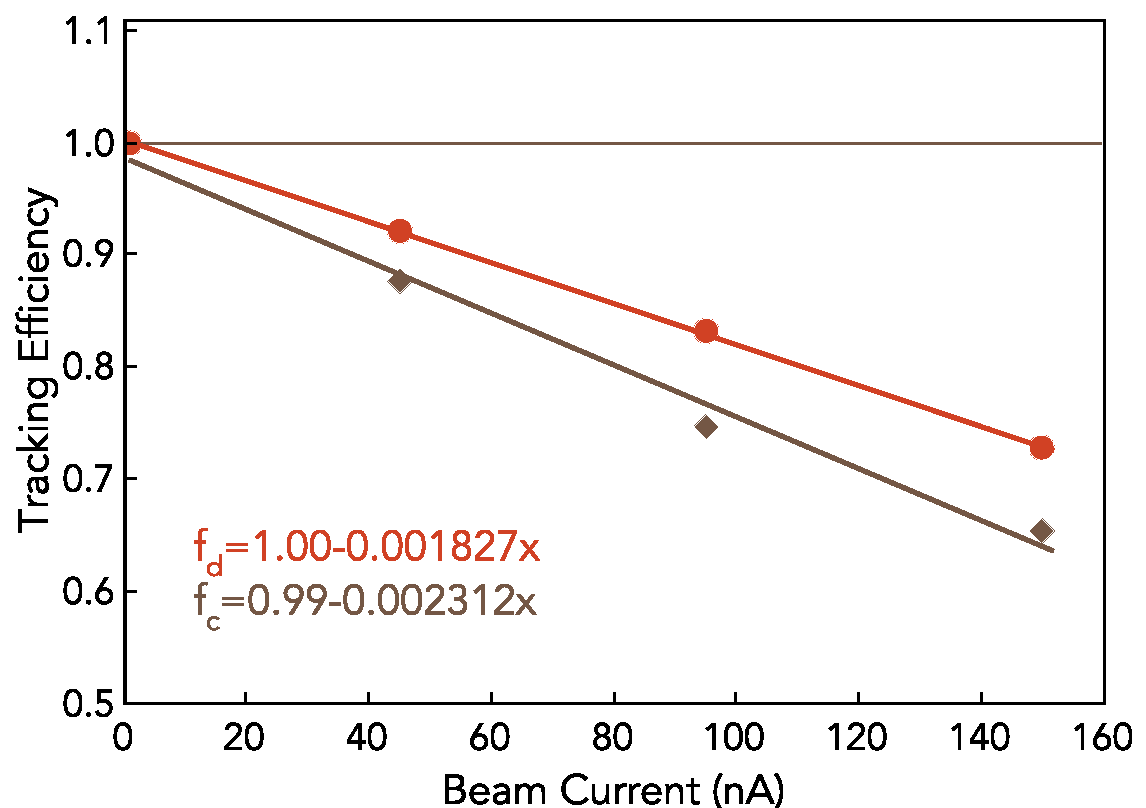
\includegraphics[width=3.1in]{images/figure_lscan_pos.pdf}
 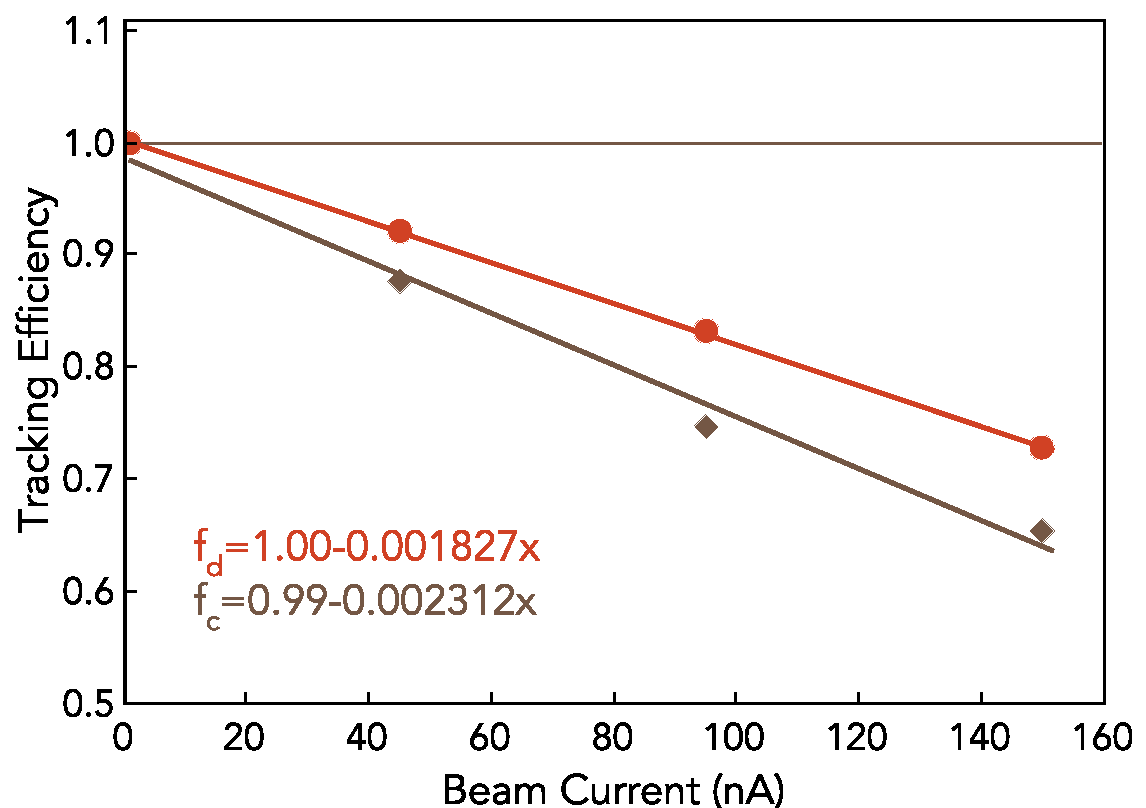
\includegraphics[width=3in]{images/figure_lscan_pos.pdf}
\caption {Tracking efficiency as a function of luminosity (beam current) for positive (a) and negative particle (b).  The efficiency is shown for
conventional algorithm running on background merged files (diamonds), and on files with merged background then de-noised with AI (circles).}
 \label{lscan::conv_dn}
 \end{center}
\end{figure}

On Figure~\ref{lscan::conv_dn} the results of analysis for different background merged files are shown. The 

\subsection{Physics Impact}

data.

\begin{figure}[!ht]
\begin{center}
 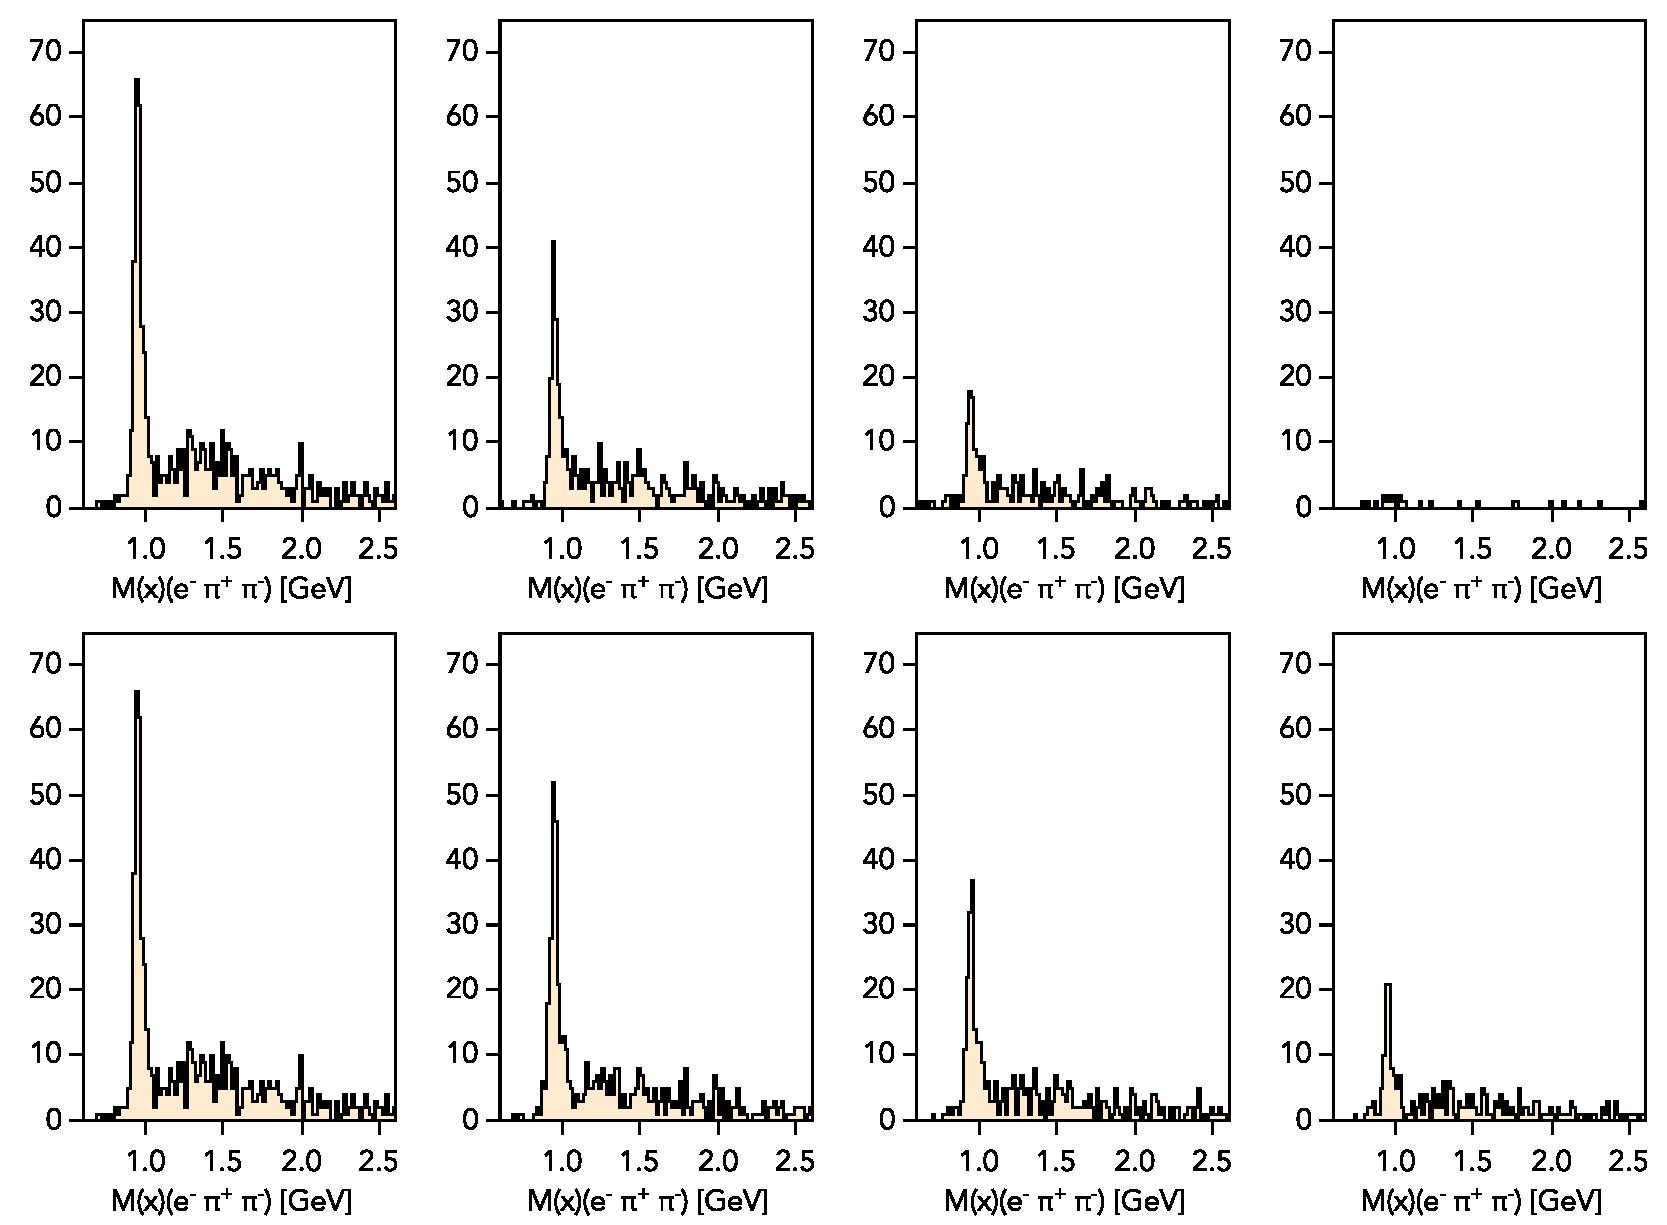
\includegraphics[width=6.1in]{images/figure_phys_conv.pdf}
\caption {Number of reconstructed protons from missing mass of $H(e \rightarrow e^\prime \pi^+\pi^-)$ for background 
merged files for  $5~nA$, $45~nA$, $95~nA$ and $150~nA$ respectively. The number of protons reconstructed by 
conventional algorithm after background merging is shown on the top row, and reconstruction after  de-noising drift 
chamber data on the bottom row.}
 \label{physics::conv_dn}
 \end{center}
\end{figure}


\begin{figure}[!ht]
\begin{center}
 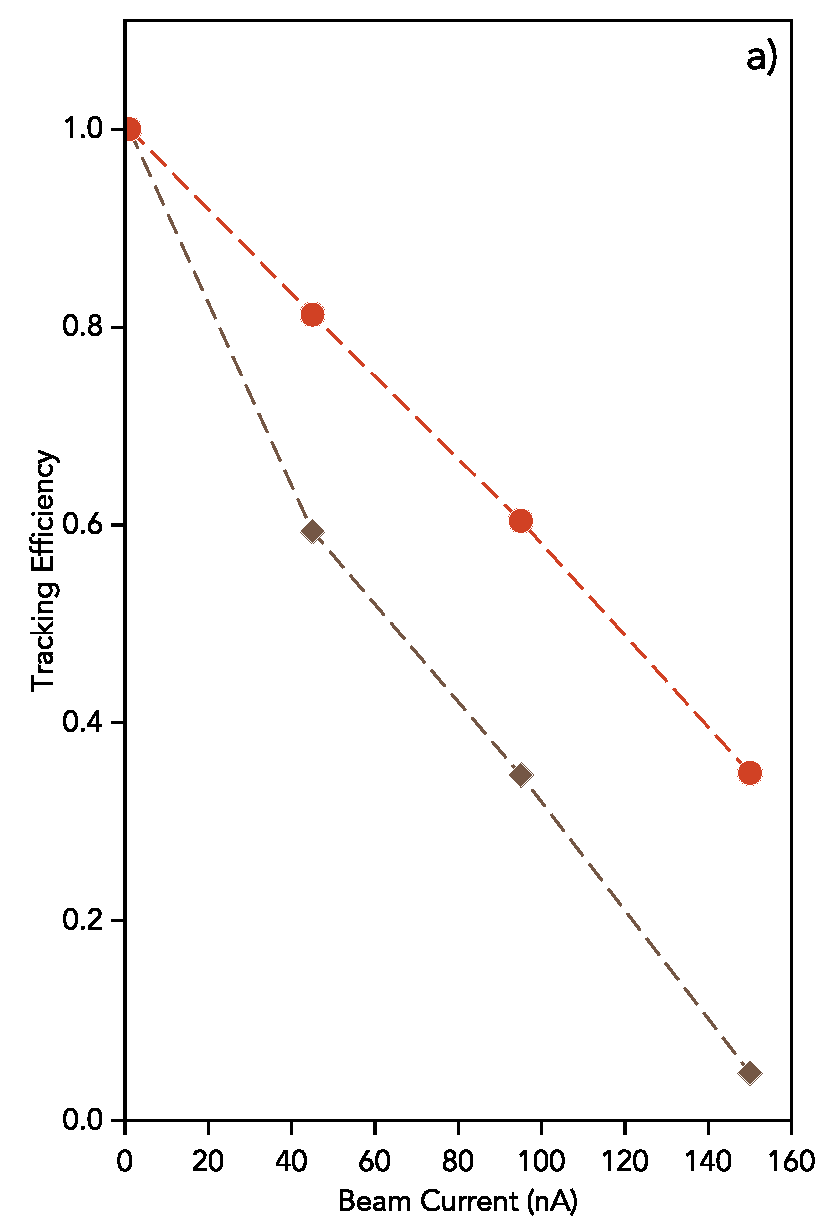
\includegraphics[width=3.1in]{images/figure_phys_scan.pdf}
 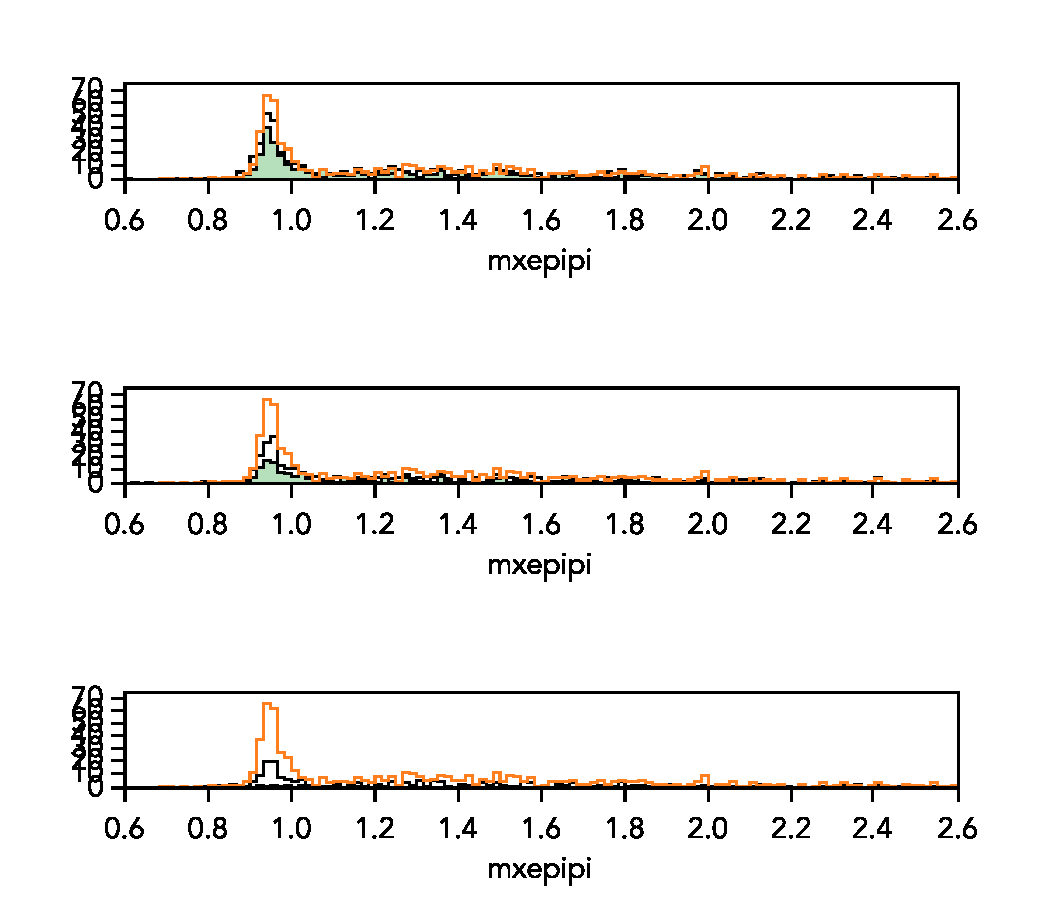
\includegraphics[width=2.5in]{images/figure_phys_conv_compare.pdf}
\caption {Number of reconstructed protons from missing mass 
of $H(e e^\prime \pi^+\pi^-)$ for background merged files for 
$5~nA$, $45~nA$, $95~nA$ and $150~nA$ respectively.}
 \label{physics::conv_dn}
 \end{center}
\end{figure}

